\documentclass[twoside]{book}

% Packages required by doxygen
\usepackage{fixltx2e}
\usepackage{calc}
\usepackage{doxygen}
\usepackage[export]{adjustbox} % also loads graphicx
\usepackage{graphicx}
\usepackage[utf8]{inputenc}
\usepackage{makeidx}
\usepackage{multicol}
\usepackage{multirow}
\PassOptionsToPackage{warn}{textcomp}
\usepackage{textcomp}
\usepackage[nointegrals]{wasysym}
\usepackage[table]{xcolor}

% Font selection
\usepackage[T1]{fontenc}
\usepackage[scaled=.90]{helvet}
\usepackage{courier}
\usepackage{amssymb}
\usepackage{sectsty}
\renewcommand{\familydefault}{\sfdefault}
\allsectionsfont{%
  \fontseries{bc}\selectfont%
  \color{darkgray}%
}
\renewcommand{\DoxyLabelFont}{%
  \fontseries{bc}\selectfont%
  \color{darkgray}%
}
\newcommand{\+}{\discretionary{\mbox{\scriptsize$\hookleftarrow$}}{}{}}

% Page & text layout
\usepackage{geometry}
\geometry{%
  a4paper,%
  top=2.5cm,%
  bottom=2.5cm,%
  left=2.5cm,%
  right=2.5cm%
}
\tolerance=750
\hfuzz=15pt
\hbadness=750
\setlength{\emergencystretch}{15pt}
\setlength{\parindent}{0cm}
\setlength{\parskip}{3ex plus 2ex minus 2ex}
\makeatletter
\renewcommand{\paragraph}{%
  \@startsection{paragraph}{4}{0ex}{-1.0ex}{1.0ex}{%
    \normalfont\normalsize\bfseries\SS@parafont%
  }%
}
\renewcommand{\subparagraph}{%
  \@startsection{subparagraph}{5}{0ex}{-1.0ex}{1.0ex}{%
    \normalfont\normalsize\bfseries\SS@subparafont%
  }%
}
\makeatother

% Headers & footers
\usepackage{fancyhdr}
\pagestyle{fancyplain}
\fancyhead[LE]{\fancyplain{}{\bfseries\thepage}}
\fancyhead[CE]{\fancyplain{}{}}
\fancyhead[RE]{\fancyplain{}{\bfseries\leftmark}}
\fancyhead[LO]{\fancyplain{}{\bfseries\rightmark}}
\fancyhead[CO]{\fancyplain{}{}}
\fancyhead[RO]{\fancyplain{}{\bfseries\thepage}}
\fancyfoot[LE]{\fancyplain{}{}}
\fancyfoot[CE]{\fancyplain{}{}}
\fancyfoot[RE]{\fancyplain{}{\bfseries\scriptsize Generated by Doxygen }}
\fancyfoot[LO]{\fancyplain{}{\bfseries\scriptsize Generated by Doxygen }}
\fancyfoot[CO]{\fancyplain{}{}}
\fancyfoot[RO]{\fancyplain{}{}}
\renewcommand{\footrulewidth}{0.4pt}
\renewcommand{\chaptermark}[1]{%
  \markboth{#1}{}%
}
\renewcommand{\sectionmark}[1]{%
  \markright{\thesection\ #1}%
}

% Indices & bibliography
\usepackage{natbib}
\usepackage[titles]{tocloft}
\setcounter{tocdepth}{3}
\setcounter{secnumdepth}{5}
\makeindex

% Hyperlinks (required, but should be loaded last)
\usepackage{ifpdf}
\ifpdf
  \usepackage[pdftex,pagebackref=true]{hyperref}
\else
  \usepackage[ps2pdf,pagebackref=true]{hyperref}
\fi
\hypersetup{%
  colorlinks=true,%
  linkcolor=blue,%
  citecolor=blue,%
  unicode%
}

% Custom commands
\newcommand{\clearemptydoublepage}{%
  \newpage{\pagestyle{empty}\cleardoublepage}%
}

\usepackage{caption}
\captionsetup{labelsep=space,justification=centering,font={bf},singlelinecheck=off,skip=4pt,position=top}

%===== C O N T E N T S =====

\begin{document}

% Titlepage & ToC
\hypersetup{pageanchor=false,
             bookmarksnumbered=true,
             pdfencoding=unicode
            }
\pagenumbering{alph}
\begin{titlepage}
\vspace*{7cm}
\begin{center}%
{\Large Word\+Counter }\\
\vspace*{1cm}
{\large Generated by Doxygen 1.8.14}\\
\end{center}
\end{titlepage}
\clearemptydoublepage
\pagenumbering{roman}
\tableofcontents
\clearemptydoublepage
\pagenumbering{arabic}
\hypersetup{pageanchor=true}

%--- Begin generated contents ---
\chapter{Class Index}
\section{Class List}
Here are the classes, structs, unions and interfaces with brief descriptions\+:\begin{DoxyCompactList}
\item\contentsline{section}{\mbox{\hyperlink{struct_word_occurrence_container_1_1_wordand_count}{Word\+Occurrence\+Container\+::\+Wordand\+Count}} \\*Structure for word and count pair. Overloads $<$ operator to use S\+TL priority queue as a min heap rather than a max heap }{\pageref{struct_word_occurrence_container_1_1_wordand_count}}{}
\item\contentsline{section}{\mbox{\hyperlink{class_word_counter}{Word\+Counter}} \\*Given a file that contains A\+S\+C\+II, counts word occurrences. Can return top ten words that occur in the file }{\pageref{class_word_counter}}{}
\item\contentsline{section}{\mbox{\hyperlink{class_word_extractor}{Word\+Extractor}} \\*Class used to extract words from file that contains A\+S\+C\+II characters }{\pageref{class_word_extractor}}{}
\item\contentsline{section}{\mbox{\hyperlink{class_word_occurrence_container}{Word\+Occurrence\+Container}} \\*Container used to keep counts of word occurrences }{\pageref{class_word_occurrence_container}}{}
\end{DoxyCompactList}

\chapter{File Index}
\section{File List}
Here is a list of all files with brief descriptions\+:\begin{DoxyCompactList}
\item\contentsline{section}{src/\mbox{\hyperlink{_word_counter_8cpp}{Word\+Counter.\+cpp}} }{\pageref{_word_counter_8cpp}}{}
\item\contentsline{section}{src/\mbox{\hyperlink{_word_counter_8hpp}{Word\+Counter.\+hpp}} }{\pageref{_word_counter_8hpp}}{}
\item\contentsline{section}{src/\mbox{\hyperlink{_word_extractor_8cpp}{Word\+Extractor.\+cpp}} }{\pageref{_word_extractor_8cpp}}{}
\item\contentsline{section}{src/\mbox{\hyperlink{_word_extractor_8hpp}{Word\+Extractor.\+hpp}} }{\pageref{_word_extractor_8hpp}}{}
\item\contentsline{section}{src/\mbox{\hyperlink{_word_occurrence_container_8cpp}{Word\+Occurrence\+Container.\+cpp}} }{\pageref{_word_occurrence_container_8cpp}}{}
\item\contentsline{section}{src/\mbox{\hyperlink{_word_occurrence_container_8hpp}{Word\+Occurrence\+Container.\+hpp}} }{\pageref{_word_occurrence_container_8hpp}}{}
\end{DoxyCompactList}

\chapter{Class Documentation}
\hypertarget{struct_word_occurrence_container_1_1_wordand_count}{}\section{Word\+Occurrence\+Container\+:\+:Wordand\+Count Struct Reference}
\label{struct_word_occurrence_container_1_1_wordand_count}\index{Word\+Occurrence\+Container\+::\+Wordand\+Count@{Word\+Occurrence\+Container\+::\+Wordand\+Count}}


structure for word and count pair. Overloads $<$ operator to use S\+TL priority queue as a min heap rather than a max heap  




Collaboration diagram for Word\+Occurrence\+Container\+:\+:Wordand\+Count\+:\nopagebreak
\begin{figure}[H]
\begin{center}
\leavevmode
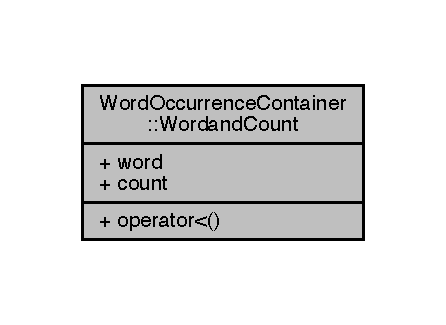
\includegraphics[width=214pt]{struct_word_occurrence_container_1_1_wordand_count__coll__graph}
\end{center}
\end{figure}
\subsection*{Public Member Functions}
\begin{DoxyCompactItemize}
\item 
bool \mbox{\hyperlink{struct_word_occurrence_container_1_1_wordand_count_a6922cc342d2df02f2786a5f1e676c7c0}{operator$<$}} (const \mbox{\hyperlink{struct_word_occurrence_container_1_1_wordand_count}{Wordand\+Count}} \&rhs) const
\end{DoxyCompactItemize}
\subsection*{Public Attributes}
\begin{DoxyCompactItemize}
\item 
std\+::string \mbox{\hyperlink{struct_word_occurrence_container_1_1_wordand_count_a7350d13d7a0942fb29f92826e6133252}{word}}
\item 
unsigned int \mbox{\hyperlink{struct_word_occurrence_container_1_1_wordand_count_ad1ee36cdf02e30c4c2de82cd47fc093b}{count}}
\end{DoxyCompactItemize}


\subsection{Detailed Description}
structure for word and count pair. Overloads $<$ operator to use S\+TL priority queue as a min heap rather than a max heap 

\subsection{Member Function Documentation}
\mbox{\Hypertarget{struct_word_occurrence_container_1_1_wordand_count_a6922cc342d2df02f2786a5f1e676c7c0}\label{struct_word_occurrence_container_1_1_wordand_count_a6922cc342d2df02f2786a5f1e676c7c0}} 
\index{Word\+Occurrence\+Container\+::\+Wordand\+Count@{Word\+Occurrence\+Container\+::\+Wordand\+Count}!operator$<$@{operator$<$}}
\index{operator$<$@{operator$<$}!Word\+Occurrence\+Container\+::\+Wordand\+Count@{Word\+Occurrence\+Container\+::\+Wordand\+Count}}
\subsubsection{\texorpdfstring{operator$<$()}{operator<()}}
{\footnotesize\ttfamily bool Word\+Occurrence\+Container\+::\+Wordand\+Count\+::operator$<$ (\begin{DoxyParamCaption}\item[{const \mbox{\hyperlink{struct_word_occurrence_container_1_1_wordand_count}{Wordand\+Count}} \&}]{rhs }\end{DoxyParamCaption}) const\hspace{0.3cm}{\ttfamily [inline]}}



\subsection{Member Data Documentation}
\mbox{\Hypertarget{struct_word_occurrence_container_1_1_wordand_count_ad1ee36cdf02e30c4c2de82cd47fc093b}\label{struct_word_occurrence_container_1_1_wordand_count_ad1ee36cdf02e30c4c2de82cd47fc093b}} 
\index{Word\+Occurrence\+Container\+::\+Wordand\+Count@{Word\+Occurrence\+Container\+::\+Wordand\+Count}!count@{count}}
\index{count@{count}!Word\+Occurrence\+Container\+::\+Wordand\+Count@{Word\+Occurrence\+Container\+::\+Wordand\+Count}}
\subsubsection{\texorpdfstring{count}{count}}
{\footnotesize\ttfamily unsigned int Word\+Occurrence\+Container\+::\+Wordand\+Count\+::count}

\mbox{\Hypertarget{struct_word_occurrence_container_1_1_wordand_count_a7350d13d7a0942fb29f92826e6133252}\label{struct_word_occurrence_container_1_1_wordand_count_a7350d13d7a0942fb29f92826e6133252}} 
\index{Word\+Occurrence\+Container\+::\+Wordand\+Count@{Word\+Occurrence\+Container\+::\+Wordand\+Count}!word@{word}}
\index{word@{word}!Word\+Occurrence\+Container\+::\+Wordand\+Count@{Word\+Occurrence\+Container\+::\+Wordand\+Count}}
\subsubsection{\texorpdfstring{word}{word}}
{\footnotesize\ttfamily std\+::string Word\+Occurrence\+Container\+::\+Wordand\+Count\+::word}



The documentation for this struct was generated from the following file\+:\begin{DoxyCompactItemize}
\item 
src/\mbox{\hyperlink{_word_occurrence_container_8hpp}{Word\+Occurrence\+Container.\+hpp}}\end{DoxyCompactItemize}

\hypertarget{class_word_counter}{}\section{Word\+Counter Class Reference}
\label{class_word_counter}\index{Word\+Counter@{Word\+Counter}}


Given a file that contains A\+S\+C\+II, counts word occurrences. Can return top ten words that occur in the file.  




{\ttfamily \#include $<$Word\+Counter.\+hpp$>$}



Collaboration diagram for Word\+Counter\+:\nopagebreak
\begin{figure}[H]
\begin{center}
\leavevmode
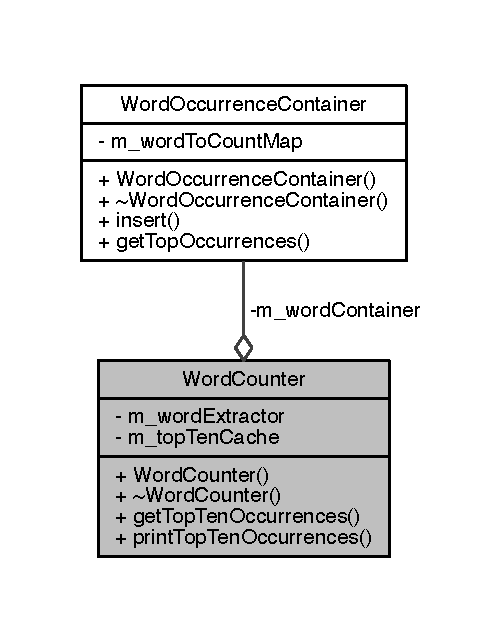
\includegraphics[width=242pt]{class_word_counter__coll__graph}
\end{center}
\end{figure}
\subsection*{Public Member Functions}
\begin{DoxyCompactItemize}
\item 
\mbox{\hyperlink{class_word_counter_affea0f9dd574ac25eb447a161b4e9c22}{Word\+Counter}} (const std\+::string \&file\+Name)
\item 
\mbox{\hyperlink{class_word_counter_ad0703060b084d90e36bb7b506c7eff94}{$\sim$\+Word\+Counter}} ()
\item 
std\+::vector$<$ std\+::pair$<$ std\+::string, unsigned int $>$ $>$ \mbox{\hyperlink{class_word_counter_a0d81dc009206dbbdddfd0fc290252855}{get\+Top\+Ten\+Occurrences}} ()
\item 
void \mbox{\hyperlink{class_word_counter_a29d681756dec9d102141c6c8a136561d}{print\+Top\+Ten\+Occurrences}} ()
\end{DoxyCompactItemize}
\subsection*{Private Attributes}
\begin{DoxyCompactItemize}
\item 
std\+::unique\+\_\+ptr$<$ \mbox{\hyperlink{class_word_extractor}{Word\+Extractor}} $>$ \mbox{\hyperlink{class_word_counter_aefb9611fa991d6e0e7dccd64403150cb}{m\+\_\+word\+Extractor}}
\item 
\mbox{\hyperlink{class_word_occurrence_container}{Word\+Occurrence\+Container}} \mbox{\hyperlink{class_word_counter_a7f867e08264a28ccfc65972bc42e409b}{m\+\_\+word\+Container}}
\item 
std\+::vector$<$ std\+::pair$<$ std\+::string, unsigned int $>$ $>$ \mbox{\hyperlink{class_word_counter_ab38650b6b6b1e07168682573f7923d24}{m\+\_\+top\+Ten\+Cache}}
\end{DoxyCompactItemize}


\subsection{Detailed Description}
Given a file that contains A\+S\+C\+II, counts word occurrences. Can return top ten words that occur in the file. 

\subsection{Constructor \& Destructor Documentation}
\mbox{\Hypertarget{class_word_counter_affea0f9dd574ac25eb447a161b4e9c22}\label{class_word_counter_affea0f9dd574ac25eb447a161b4e9c22}} 
\index{Word\+Counter@{Word\+Counter}!Word\+Counter@{Word\+Counter}}
\index{Word\+Counter@{Word\+Counter}!Word\+Counter@{Word\+Counter}}
\subsubsection{\texorpdfstring{Word\+Counter()}{WordCounter()}}
{\footnotesize\ttfamily Word\+Counter\+::\+Word\+Counter (\begin{DoxyParamCaption}\item[{const std\+::string \&}]{file\+Name }\end{DoxyParamCaption})}

Constructs a \mbox{\hyperlink{class_word_counter}{Word\+Counter}} 
\begin{DoxyParams}{Parameters}
{\em file\+Name} & -\/ File to be read \\
\hline
\end{DoxyParams}

\begin{DoxyExceptions}{Exceptions}
{\em throws} & std\+::invalid\+\_\+argument if file cannot be opened \\
\hline
\end{DoxyExceptions}
\mbox{\Hypertarget{class_word_counter_ad0703060b084d90e36bb7b506c7eff94}\label{class_word_counter_ad0703060b084d90e36bb7b506c7eff94}} 
\index{Word\+Counter@{Word\+Counter}!````~Word\+Counter@{$\sim$\+Word\+Counter}}
\index{````~Word\+Counter@{$\sim$\+Word\+Counter}!Word\+Counter@{Word\+Counter}}
\subsubsection{\texorpdfstring{$\sim$\+Word\+Counter()}{~WordCounter()}}
{\footnotesize\ttfamily Word\+Counter\+::$\sim$\+Word\+Counter (\begin{DoxyParamCaption}{ }\end{DoxyParamCaption})}



\subsection{Member Function Documentation}
\mbox{\Hypertarget{class_word_counter_a0d81dc009206dbbdddfd0fc290252855}\label{class_word_counter_a0d81dc009206dbbdddfd0fc290252855}} 
\index{Word\+Counter@{Word\+Counter}!get\+Top\+Ten\+Occurrences@{get\+Top\+Ten\+Occurrences}}
\index{get\+Top\+Ten\+Occurrences@{get\+Top\+Ten\+Occurrences}!Word\+Counter@{Word\+Counter}}
\subsubsection{\texorpdfstring{get\+Top\+Ten\+Occurrences()}{getTopTenOccurrences()}}
{\footnotesize\ttfamily std\+::vector$<$ std\+::pair$<$ std\+::string, unsigned int $>$ $>$ Word\+Counter\+::get\+Top\+Ten\+Occurrences (\begin{DoxyParamCaption}{ }\end{DoxyParamCaption})}

\mbox{\Hypertarget{class_word_counter_a29d681756dec9d102141c6c8a136561d}\label{class_word_counter_a29d681756dec9d102141c6c8a136561d}} 
\index{Word\+Counter@{Word\+Counter}!print\+Top\+Ten\+Occurrences@{print\+Top\+Ten\+Occurrences}}
\index{print\+Top\+Ten\+Occurrences@{print\+Top\+Ten\+Occurrences}!Word\+Counter@{Word\+Counter}}
\subsubsection{\texorpdfstring{print\+Top\+Ten\+Occurrences()}{printTopTenOccurrences()}}
{\footnotesize\ttfamily void Word\+Counter\+::print\+Top\+Ten\+Occurrences (\begin{DoxyParamCaption}{ }\end{DoxyParamCaption})}



\subsection{Member Data Documentation}
\mbox{\Hypertarget{class_word_counter_ab38650b6b6b1e07168682573f7923d24}\label{class_word_counter_ab38650b6b6b1e07168682573f7923d24}} 
\index{Word\+Counter@{Word\+Counter}!m\+\_\+top\+Ten\+Cache@{m\+\_\+top\+Ten\+Cache}}
\index{m\+\_\+top\+Ten\+Cache@{m\+\_\+top\+Ten\+Cache}!Word\+Counter@{Word\+Counter}}
\subsubsection{\texorpdfstring{m\+\_\+top\+Ten\+Cache}{m\_topTenCache}}
{\footnotesize\ttfamily std\+::vector$<$std\+::pair$<$std\+::string, unsigned int$>$ $>$ Word\+Counter\+::m\+\_\+top\+Ten\+Cache\hspace{0.3cm}{\ttfamily [private]}}

\mbox{\Hypertarget{class_word_counter_a7f867e08264a28ccfc65972bc42e409b}\label{class_word_counter_a7f867e08264a28ccfc65972bc42e409b}} 
\index{Word\+Counter@{Word\+Counter}!m\+\_\+word\+Container@{m\+\_\+word\+Container}}
\index{m\+\_\+word\+Container@{m\+\_\+word\+Container}!Word\+Counter@{Word\+Counter}}
\subsubsection{\texorpdfstring{m\+\_\+word\+Container}{m\_wordContainer}}
{\footnotesize\ttfamily \mbox{\hyperlink{class_word_occurrence_container}{Word\+Occurrence\+Container}} Word\+Counter\+::m\+\_\+word\+Container\hspace{0.3cm}{\ttfamily [private]}}

Container used to keep track of occurrences of words \mbox{\Hypertarget{class_word_counter_aefb9611fa991d6e0e7dccd64403150cb}\label{class_word_counter_aefb9611fa991d6e0e7dccd64403150cb}} 
\index{Word\+Counter@{Word\+Counter}!m\+\_\+word\+Extractor@{m\+\_\+word\+Extractor}}
\index{m\+\_\+word\+Extractor@{m\+\_\+word\+Extractor}!Word\+Counter@{Word\+Counter}}
\subsubsection{\texorpdfstring{m\+\_\+word\+Extractor}{m\_wordExtractor}}
{\footnotesize\ttfamily std\+::unique\+\_\+ptr$<$\mbox{\hyperlink{class_word_extractor}{Word\+Extractor}}$>$ Word\+Counter\+::m\+\_\+word\+Extractor\hspace{0.3cm}{\ttfamily [private]}}

object used to extract words from file 

The documentation for this class was generated from the following files\+:\begin{DoxyCompactItemize}
\item 
src/\mbox{\hyperlink{_word_counter_8hpp}{Word\+Counter.\+hpp}}\item 
src/\mbox{\hyperlink{_word_counter_8cpp}{Word\+Counter.\+cpp}}\end{DoxyCompactItemize}

\hypertarget{class_word_extractor}{}\section{Word\+Extractor Class Reference}
\label{class_word_extractor}\index{Word\+Extractor@{Word\+Extractor}}


Class used to extract words from file that contains A\+S\+C\+II characters.  




{\ttfamily \#include $<$Word\+Extractor.\+hpp$>$}



Collaboration diagram for Word\+Extractor\+:
\nopagebreak
\begin{figure}[H]
\begin{center}
\leavevmode
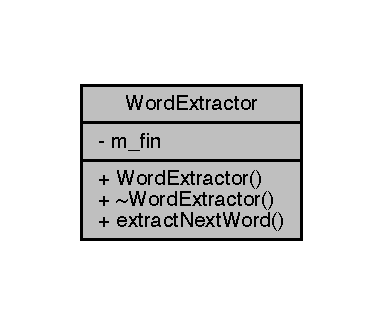
\includegraphics[width=184pt]{class_word_extractor__coll__graph}
\end{center}
\end{figure}
\subsection*{Public Member Functions}
\begin{DoxyCompactItemize}
\item 
\mbox{\hyperlink{class_word_extractor_ad49ed8d220bc9cd36f3b0a285d52a081}{Word\+Extractor}} (const std\+::string \&file\+Name)
\item 
\mbox{\hyperlink{class_word_extractor_a20476de5cb146afd9bc318a629157a9c}{$\sim$\+Word\+Extractor}} ()
\item 
std\+::string \mbox{\hyperlink{class_word_extractor_aae86b87d65bcfe432ec50c88fec4f464}{extract\+Next\+Word}} ()
\begin{DoxyCompactList}\small\item\em Extracts the next word. Ignores punctuation (eg. it\textquotesingle{}s = its) If multiple words are concatenated together with a character like hyphen(-\/) or underscore(\+\_\+) it will count them as seperate words. \end{DoxyCompactList}\end{DoxyCompactItemize}
\subsection*{Private Attributes}
\begin{DoxyCompactItemize}
\item 
std\+::ifstream \mbox{\hyperlink{class_word_extractor_af189c1c3a30c9e06d5bda3ac358d0963}{m\+\_\+fin}}
\end{DoxyCompactItemize}


\subsection{Detailed Description}
Class used to extract words from file that contains A\+S\+C\+II characters. 

\subsection{Constructor \& Destructor Documentation}
\mbox{\Hypertarget{class_word_extractor_ad49ed8d220bc9cd36f3b0a285d52a081}\label{class_word_extractor_ad49ed8d220bc9cd36f3b0a285d52a081}} 
\index{Word\+Extractor@{Word\+Extractor}!Word\+Extractor@{Word\+Extractor}}
\index{Word\+Extractor@{Word\+Extractor}!Word\+Extractor@{Word\+Extractor}}
\subsubsection{\texorpdfstring{Word\+Extractor()}{WordExtractor()}}
{\footnotesize\ttfamily Word\+Extractor\+::\+Word\+Extractor (\begin{DoxyParamCaption}\item[{const std\+::string \&}]{file\+Name }\end{DoxyParamCaption})}

Opens file for reading. 
\begin{DoxyParams}{Parameters}
{\em file\+Name} & -\/ File to be read. \\
\hline
\end{DoxyParams}
\mbox{\Hypertarget{class_word_extractor_a20476de5cb146afd9bc318a629157a9c}\label{class_word_extractor_a20476de5cb146afd9bc318a629157a9c}} 
\index{Word\+Extractor@{Word\+Extractor}!````~Word\+Extractor@{$\sim$\+Word\+Extractor}}
\index{````~Word\+Extractor@{$\sim$\+Word\+Extractor}!Word\+Extractor@{Word\+Extractor}}
\subsubsection{\texorpdfstring{$\sim$\+Word\+Extractor()}{~WordExtractor()}}
{\footnotesize\ttfamily Word\+Extractor\+::$\sim$\+Word\+Extractor (\begin{DoxyParamCaption}{ }\end{DoxyParamCaption})}

Closes file 

\subsection{Member Function Documentation}
\mbox{\Hypertarget{class_word_extractor_aae86b87d65bcfe432ec50c88fec4f464}\label{class_word_extractor_aae86b87d65bcfe432ec50c88fec4f464}} 
\index{Word\+Extractor@{Word\+Extractor}!extract\+Next\+Word@{extract\+Next\+Word}}
\index{extract\+Next\+Word@{extract\+Next\+Word}!Word\+Extractor@{Word\+Extractor}}
\subsubsection{\texorpdfstring{extract\+Next\+Word()}{extractNextWord()}}
{\footnotesize\ttfamily std\+::string Word\+Extractor\+::extract\+Next\+Word (\begin{DoxyParamCaption}{ }\end{DoxyParamCaption})}



Extracts the next word. Ignores punctuation (eg. it\textquotesingle{}s = its) If multiple words are concatenated together with a character like hyphen(-\/) or underscore(\+\_\+) it will count them as seperate words. 

\begin{DoxyReturn}{Returns}
Extracted word. 
\end{DoxyReturn}


\subsection{Member Data Documentation}
\mbox{\Hypertarget{class_word_extractor_af189c1c3a30c9e06d5bda3ac358d0963}\label{class_word_extractor_af189c1c3a30c9e06d5bda3ac358d0963}} 
\index{Word\+Extractor@{Word\+Extractor}!m\+\_\+fin@{m\+\_\+fin}}
\index{m\+\_\+fin@{m\+\_\+fin}!Word\+Extractor@{Word\+Extractor}}
\subsubsection{\texorpdfstring{m\+\_\+fin}{m\_fin}}
{\footnotesize\ttfamily std\+::ifstream Word\+Extractor\+::m\+\_\+fin\hspace{0.3cm}{\ttfamily [private]}}



The documentation for this class was generated from the following files\+:\begin{DoxyCompactItemize}
\item 
src/\mbox{\hyperlink{_word_extractor_8hpp}{Word\+Extractor.\+hpp}}\item 
src/\mbox{\hyperlink{_word_extractor_8cpp}{Word\+Extractor.\+cpp}}\end{DoxyCompactItemize}

\hypertarget{class_word_occurrence_container}{}\section{Word\+Occurrence\+Container Class Reference}
\label{class_word_occurrence_container}\index{Word\+Occurrence\+Container@{Word\+Occurrence\+Container}}


Container used to keep counts of word occurrences.  




{\ttfamily \#include $<$Word\+Occurrence\+Container.\+hpp$>$}



Collaboration diagram for Word\+Occurrence\+Container\+:\nopagebreak
\begin{figure}[H]
\begin{center}
\leavevmode
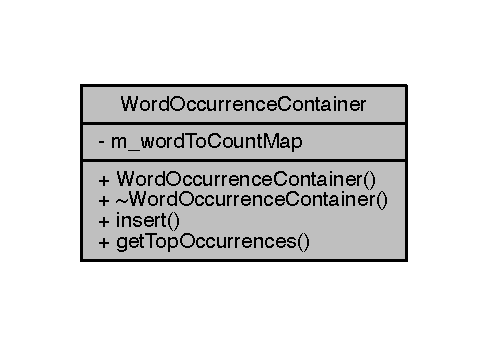
\includegraphics[width=234pt]{class_word_occurrence_container__coll__graph}
\end{center}
\end{figure}
\subsection*{Classes}
\begin{DoxyCompactItemize}
\item 
struct \mbox{\hyperlink{struct_word_occurrence_container_1_1_wordand_count}{Wordand\+Count}}
\begin{DoxyCompactList}\small\item\em structure for word and count pair. Overloads $<$ operator to use S\+TL priority queue as a min heap rather than a max heap \end{DoxyCompactList}\end{DoxyCompactItemize}
\subsection*{Public Member Functions}
\begin{DoxyCompactItemize}
\item 
\mbox{\hyperlink{class_word_occurrence_container_a777151c21ae2e8d60fbdecb000cd2f44}{Word\+Occurrence\+Container}} ()
\item 
\mbox{\hyperlink{class_word_occurrence_container_a96a671f07750218a9325a8cab89288ef}{$\sim$\+Word\+Occurrence\+Container}} ()
\item 
void \mbox{\hyperlink{class_word_occurrence_container_a3ea24956cdbd599593bd4c0256cf9d15}{insert}} (const std\+::string \&word)
\begin{DoxyCompactList}\small\item\em Inserts a word into the \mbox{\hyperlink{class_word_occurrence_container}{Word\+Occurrence\+Container}}. Assumes input string is a word and not empty. \end{DoxyCompactList}\item 
std\+::vector$<$ std\+::pair$<$ std\+::string, unsigned int $>$ $>$ \mbox{\hyperlink{class_word_occurrence_container_aa4402285c14c3d282aa34c62934260e1}{get\+Top\+Occurrences}} (const unsigned int \&n)
\begin{DoxyCompactList}\small\item\em Gets the top n words that occur the most. \end{DoxyCompactList}\end{DoxyCompactItemize}
\subsection*{Private Attributes}
\begin{DoxyCompactItemize}
\item 
std\+::unordered\+\_\+map$<$ std\+::string, unsigned int $>$ \mbox{\hyperlink{class_word_occurrence_container_ab2f0abb68fe94056659c7a1e0f919ae2}{m\+\_\+word\+To\+Count\+Map}}
\end{DoxyCompactItemize}


\subsection{Detailed Description}
Container used to keep counts of word occurrences. 

\subsection{Constructor \& Destructor Documentation}
\mbox{\Hypertarget{class_word_occurrence_container_a777151c21ae2e8d60fbdecb000cd2f44}\label{class_word_occurrence_container_a777151c21ae2e8d60fbdecb000cd2f44}} 
\index{Word\+Occurrence\+Container@{Word\+Occurrence\+Container}!Word\+Occurrence\+Container@{Word\+Occurrence\+Container}}
\index{Word\+Occurrence\+Container@{Word\+Occurrence\+Container}!Word\+Occurrence\+Container@{Word\+Occurrence\+Container}}
\subsubsection{\texorpdfstring{Word\+Occurrence\+Container()}{WordOccurrenceContainer()}}
{\footnotesize\ttfamily Word\+Occurrence\+Container\+::\+Word\+Occurrence\+Container (\begin{DoxyParamCaption}{ }\end{DoxyParamCaption})}

\mbox{\Hypertarget{class_word_occurrence_container_a96a671f07750218a9325a8cab89288ef}\label{class_word_occurrence_container_a96a671f07750218a9325a8cab89288ef}} 
\index{Word\+Occurrence\+Container@{Word\+Occurrence\+Container}!````~Word\+Occurrence\+Container@{$\sim$\+Word\+Occurrence\+Container}}
\index{````~Word\+Occurrence\+Container@{$\sim$\+Word\+Occurrence\+Container}!Word\+Occurrence\+Container@{Word\+Occurrence\+Container}}
\subsubsection{\texorpdfstring{$\sim$\+Word\+Occurrence\+Container()}{~WordOccurrenceContainer()}}
{\footnotesize\ttfamily Word\+Occurrence\+Container\+::$\sim$\+Word\+Occurrence\+Container (\begin{DoxyParamCaption}{ }\end{DoxyParamCaption})}



\subsection{Member Function Documentation}
\mbox{\Hypertarget{class_word_occurrence_container_aa4402285c14c3d282aa34c62934260e1}\label{class_word_occurrence_container_aa4402285c14c3d282aa34c62934260e1}} 
\index{Word\+Occurrence\+Container@{Word\+Occurrence\+Container}!get\+Top\+Occurrences@{get\+Top\+Occurrences}}
\index{get\+Top\+Occurrences@{get\+Top\+Occurrences}!Word\+Occurrence\+Container@{Word\+Occurrence\+Container}}
\subsubsection{\texorpdfstring{get\+Top\+Occurrences()}{getTopOccurrences()}}
{\footnotesize\ttfamily vector$<$ pair$<$ string, unsigned int $>$ $>$ Word\+Occurrence\+Container\+::get\+Top\+Occurrences (\begin{DoxyParamCaption}\item[{const unsigned int \&}]{n }\end{DoxyParamCaption})}



Gets the top n words that occur the most. 


\begin{DoxyParams}{Parameters}
{\em n} & -\/ top n words that occur. \\
\hline
\end{DoxyParams}
\begin{DoxyReturn}{Returns}
Vector of pairs where first is the word and second is the count. 
\end{DoxyReturn}
\mbox{\Hypertarget{class_word_occurrence_container_a3ea24956cdbd599593bd4c0256cf9d15}\label{class_word_occurrence_container_a3ea24956cdbd599593bd4c0256cf9d15}} 
\index{Word\+Occurrence\+Container@{Word\+Occurrence\+Container}!insert@{insert}}
\index{insert@{insert}!Word\+Occurrence\+Container@{Word\+Occurrence\+Container}}
\subsubsection{\texorpdfstring{insert()}{insert()}}
{\footnotesize\ttfamily void Word\+Occurrence\+Container\+::insert (\begin{DoxyParamCaption}\item[{const std\+::string \&}]{word }\end{DoxyParamCaption})}



Inserts a word into the \mbox{\hyperlink{class_word_occurrence_container}{Word\+Occurrence\+Container}}. Assumes input string is a word and not empty. 


\begin{DoxyParams}{Parameters}
{\em word} & -\/ The word that will be inserted. \\
\hline
\end{DoxyParams}


\subsection{Member Data Documentation}
\mbox{\Hypertarget{class_word_occurrence_container_ab2f0abb68fe94056659c7a1e0f919ae2}\label{class_word_occurrence_container_ab2f0abb68fe94056659c7a1e0f919ae2}} 
\index{Word\+Occurrence\+Container@{Word\+Occurrence\+Container}!m\+\_\+word\+To\+Count\+Map@{m\+\_\+word\+To\+Count\+Map}}
\index{m\+\_\+word\+To\+Count\+Map@{m\+\_\+word\+To\+Count\+Map}!Word\+Occurrence\+Container@{Word\+Occurrence\+Container}}
\subsubsection{\texorpdfstring{m\+\_\+word\+To\+Count\+Map}{m\_wordToCountMap}}
{\footnotesize\ttfamily std\+::unordered\+\_\+map$<$std\+::string, unsigned int$>$ Word\+Occurrence\+Container\+::m\+\_\+word\+To\+Count\+Map\hspace{0.3cm}{\ttfamily [private]}}

Hash\+Map that maps word to count 

The documentation for this class was generated from the following files\+:\begin{DoxyCompactItemize}
\item 
src/\mbox{\hyperlink{_word_occurrence_container_8hpp}{Word\+Occurrence\+Container.\+hpp}}\item 
src/\mbox{\hyperlink{_word_occurrence_container_8cpp}{Word\+Occurrence\+Container.\+cpp}}\end{DoxyCompactItemize}

\chapter{File Documentation}
\hypertarget{_word_counter_8cpp}{}\section{src/\+Word\+Counter.cpp File Reference}
\label{_word_counter_8cpp}\index{src/\+Word\+Counter.\+cpp@{src/\+Word\+Counter.\+cpp}}
{\ttfamily \#include $<$iostream$>$}\newline
{\ttfamily \#include \char`\"{}Word\+Counter.\+hpp\char`\"{}}\newline
Include dependency graph for Word\+Counter.\+cpp\+:\nopagebreak
\begin{figure}[H]
\begin{center}
\leavevmode
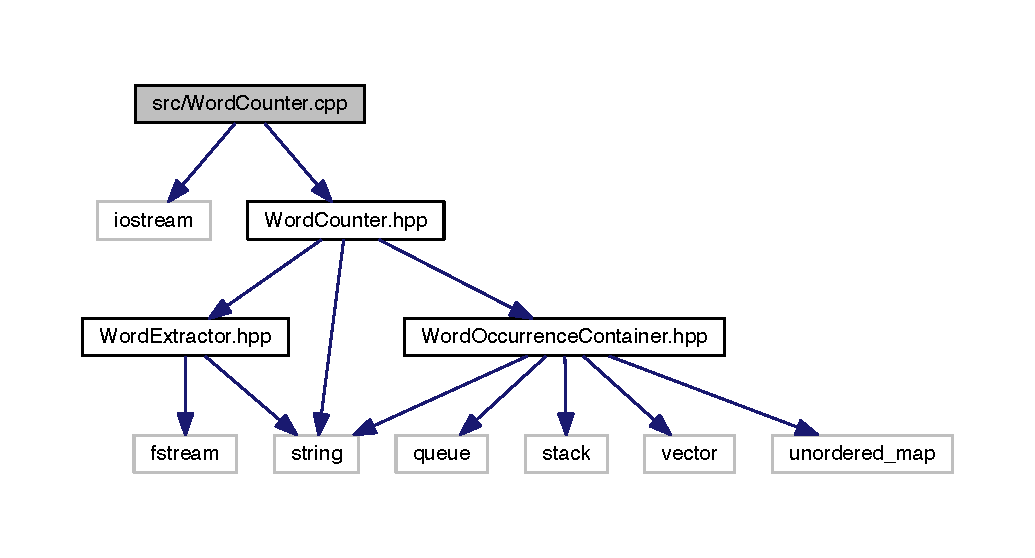
\includegraphics[width=350pt]{_word_counter_8cpp__incl}
\end{center}
\end{figure}

\hypertarget{_word_counter_8hpp}{}\section{src/\+Word\+Counter.hpp File Reference}
\label{_word_counter_8hpp}\index{src/\+Word\+Counter.\+hpp@{src/\+Word\+Counter.\+hpp}}
{\ttfamily \#include $<$string$>$}\newline
{\ttfamily \#include \char`\"{}Word\+Extractor.\+hpp\char`\"{}}\newline
{\ttfamily \#include \char`\"{}Word\+Occurrence\+Container.\+hpp\char`\"{}}\newline
Include dependency graph for Word\+Counter.\+hpp\+:\nopagebreak
\begin{figure}[H]
\begin{center}
\leavevmode
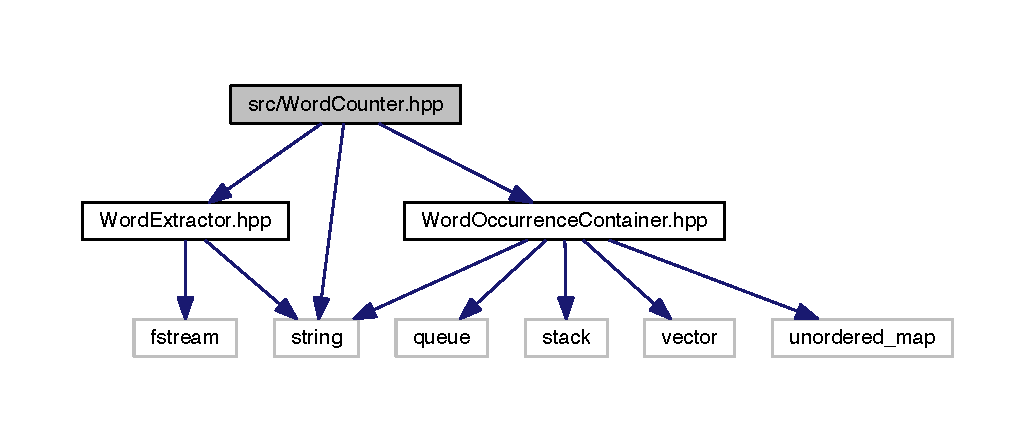
\includegraphics[width=350pt]{_word_counter_8hpp__incl}
\end{center}
\end{figure}
This graph shows which files directly or indirectly include this file\+:\nopagebreak
\begin{figure}[H]
\begin{center}
\leavevmode
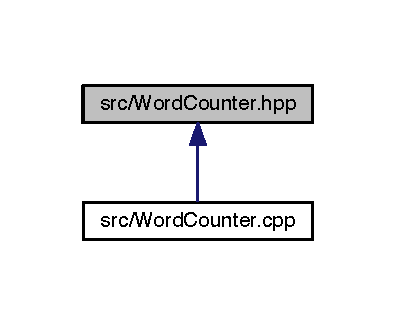
\includegraphics[width=190pt]{_word_counter_8hpp__dep__incl}
\end{center}
\end{figure}
\subsection*{Classes}
\begin{DoxyCompactItemize}
\item 
class \mbox{\hyperlink{class_word_counter}{Word\+Counter}}
\begin{DoxyCompactList}\small\item\em Given a file that contains A\+S\+C\+II, counts word occurrences. Can return top ten words that occur in the file. \end{DoxyCompactList}\end{DoxyCompactItemize}

\hypertarget{_word_extractor_8cpp}{}\section{src/\+Word\+Extractor.cpp File Reference}
\label{_word_extractor_8cpp}\index{src/\+Word\+Extractor.\+cpp@{src/\+Word\+Extractor.\+cpp}}
{\ttfamily \#include $<$iostream$>$}\newline
{\ttfamily \#include \char`\"{}Word\+Extractor.\+hpp\char`\"{}}\newline
Include dependency graph for Word\+Extractor.\+cpp\+:\nopagebreak
\begin{figure}[H]
\begin{center}
\leavevmode
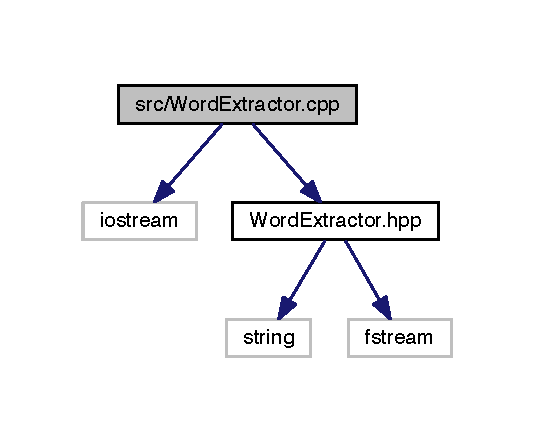
\includegraphics[width=256pt]{_word_extractor_8cpp__incl}
\end{center}
\end{figure}

\hypertarget{_word_extractor_8hpp}{}\section{src/\+Word\+Extractor.hpp File Reference}
\label{_word_extractor_8hpp}\index{src/\+Word\+Extractor.\+hpp@{src/\+Word\+Extractor.\+hpp}}
{\ttfamily \#include $<$string$>$}\newline
{\ttfamily \#include $<$fstream$>$}\newline
Include dependency graph for Word\+Extractor.\+hpp\+:\nopagebreak
\begin{figure}[H]
\begin{center}
\leavevmode
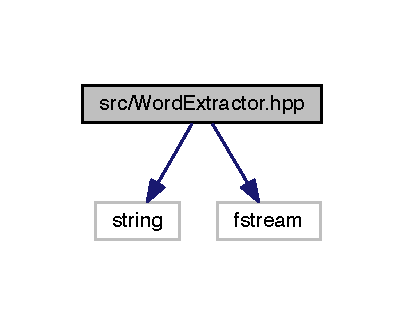
\includegraphics[width=194pt]{_word_extractor_8hpp__incl}
\end{center}
\end{figure}
This graph shows which files directly or indirectly include this file\+:\nopagebreak
\begin{figure}[H]
\begin{center}
\leavevmode
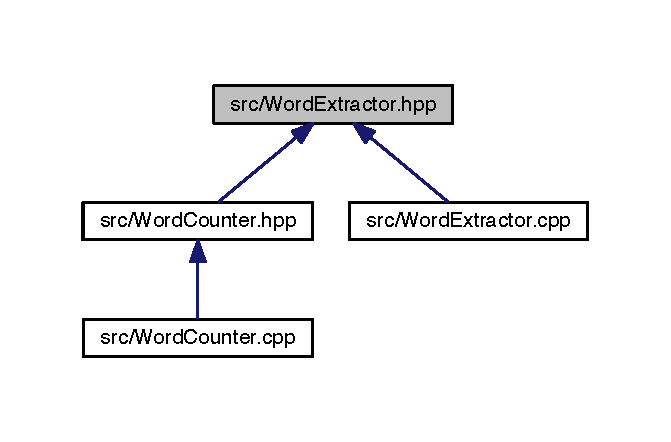
\includegraphics[width=322pt]{_word_extractor_8hpp__dep__incl}
\end{center}
\end{figure}
\subsection*{Classes}
\begin{DoxyCompactItemize}
\item 
class \mbox{\hyperlink{class_word_extractor}{Word\+Extractor}}
\begin{DoxyCompactList}\small\item\em Class used to extract words from file that contains A\+S\+C\+II characters. \end{DoxyCompactList}\end{DoxyCompactItemize}

\hypertarget{_word_occurrence_container_8cpp}{}\section{src/\+Word\+Occurrence\+Container.cpp File Reference}
\label{_word_occurrence_container_8cpp}\index{src/\+Word\+Occurrence\+Container.\+cpp@{src/\+Word\+Occurrence\+Container.\+cpp}}
{\ttfamily \#include $<$iostream$>$}\newline
{\ttfamily \#include $<$stack$>$}\newline
{\ttfamily \#include \char`\"{}Word\+Occurrence\+Container.\+hpp\char`\"{}}\newline
Include dependency graph for Word\+Occurrence\+Container.\+cpp\+:\nopagebreak
\begin{figure}[H]
\begin{center}
\leavevmode
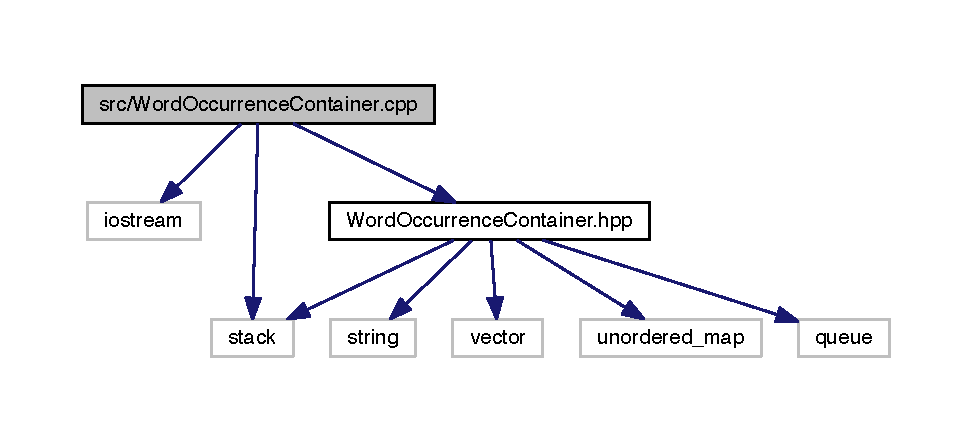
\includegraphics[width=350pt]{_word_occurrence_container_8cpp__incl}
\end{center}
\end{figure}

\hypertarget{_word_occurrence_container_8hpp}{}\section{src/\+Word\+Occurrence\+Container.hpp File Reference}
\label{_word_occurrence_container_8hpp}\index{src/\+Word\+Occurrence\+Container.\+hpp@{src/\+Word\+Occurrence\+Container.\+hpp}}
{\ttfamily \#include $<$string$>$}\newline
{\ttfamily \#include $<$vector$>$}\newline
{\ttfamily \#include $<$unordered\+\_\+map$>$}\newline
{\ttfamily \#include $<$queue$>$}\newline
{\ttfamily \#include $<$stack$>$}\newline
Include dependency graph for Word\+Occurrence\+Container.\+hpp\+:\nopagebreak
\begin{figure}[H]
\begin{center}
\leavevmode
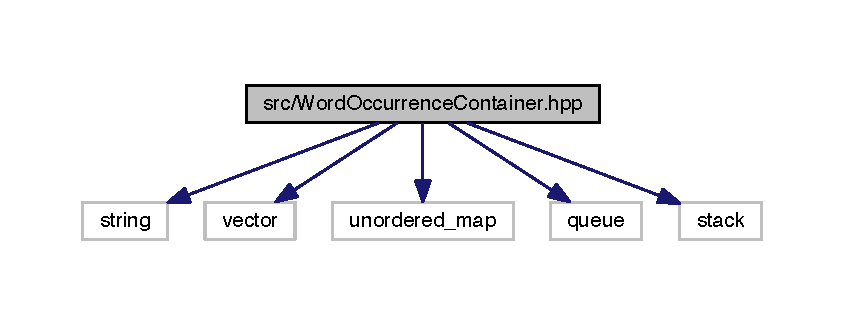
\includegraphics[width=350pt]{_word_occurrence_container_8hpp__incl}
\end{center}
\end{figure}
This graph shows which files directly or indirectly include this file\+:\nopagebreak
\begin{figure}[H]
\begin{center}
\leavevmode
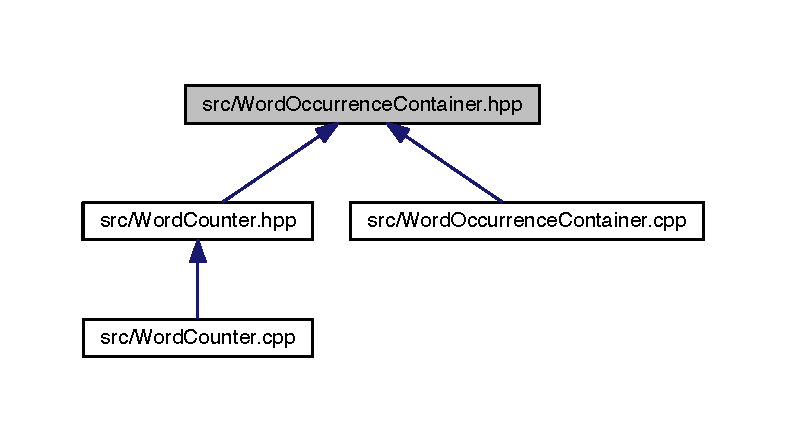
\includegraphics[width=350pt]{_word_occurrence_container_8hpp__dep__incl}
\end{center}
\end{figure}
\subsection*{Classes}
\begin{DoxyCompactItemize}
\item 
class \mbox{\hyperlink{class_word_occurrence_container}{Word\+Occurrence\+Container}}
\begin{DoxyCompactList}\small\item\em Container used to keep counts of word occurrences. \end{DoxyCompactList}\item 
struct \mbox{\hyperlink{struct_word_occurrence_container_1_1_wordand_count}{Word\+Occurrence\+Container\+::\+Wordand\+Count}}
\begin{DoxyCompactList}\small\item\em structure for word and count pair. Overloads $<$ operator to use S\+TL priority queue as a min heap rather than a max heap \end{DoxyCompactList}\end{DoxyCompactItemize}

%--- End generated contents ---

% Index
\backmatter
\newpage
\phantomsection
\clearemptydoublepage
\addcontentsline{toc}{chapter}{Index}
\printindex

\end{document}
